% This file was created with tikzplotlib v0.10.1.
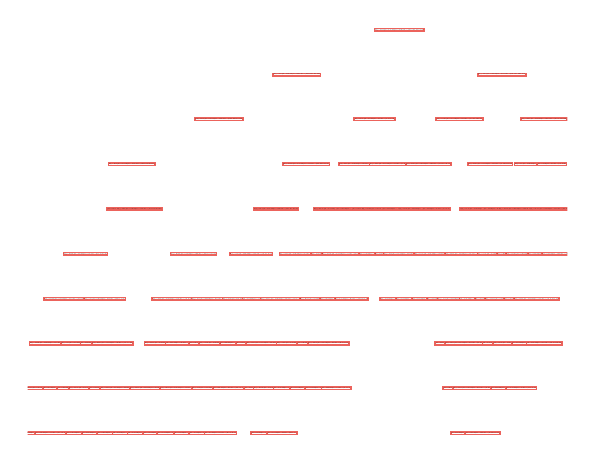
\begin{tikzpicture}

\definecolor{darkgray176}{RGB}{176,176,176}
\definecolor{tomato2369992}{RGB}{236,99,92}

\begin{axis}[
hide x axis,
hide y axis,
tick align=outside,
tick pos=left,
x grid style={darkgray176},
xmin=0, xmax=1,
xtick style={color=black},
y grid style={darkgray176},
ymin=0, ymax=1,
ytick style={color=black}
]
\draw (axis cs:0.0142857142857143,0.05) node[
  scale=0.05,
  fill=white,
  draw=tomato2369992,
  line width=0.6pt,
  inner sep=3.6pt,
  text=black,
  rotate=0.0,
  align=center
]{gini = 0.483
samples = 27
value = [11, 0, 0, 16]};
\draw (axis cs:0.0428571428571429,0.05) node[
  scale=0.05,
  fill=white,
  draw=tomato2369992,
  line width=0.6pt,
  inner sep=3.6pt,
  text=black,
  rotate=0.0,
  align=center
]{gini = 0.328
samples = 653
value = [519, 3, 0, 131]};
\draw (axis cs:0.1,0.05) node[
  scale=0.05,
  fill=white,
  draw=tomato2369992,
  line width=0.6pt,
  inner sep=3.6pt,
  text=black,
  rotate=0.0,
  align=center
]{gini = 0.329
samples = 241
value = [193, 4, 3, 41]};
\draw (axis cs:0.128571428571429,0.05) node[
  scale=0.05,
  fill=white,
  draw=tomato2369992,
  line width=0.6pt,
  inner sep=3.6pt,
  text=black,
  rotate=0.0,
  align=center
]{gini = 0.477
samples = 112
value = [68, 0, 0, 44]};
\draw (axis cs:0.157142857142857,0.05) node[
  scale=0.05,
  fill=white,
  draw=tomato2369992,
  line width=0.6pt,
  inner sep=3.6pt,
  text=black,
  rotate=0.0,
  align=center
]{gini = 0.487
samples = 148
value = [88, 1, 0, 59]};
\draw (axis cs:0.185714285714286,0.05) node[
  scale=0.05,
  fill=white,
  draw=tomato2369992,
  line width=0.6pt,
  inner sep=3.6pt,
  text=black,
  rotate=0.0,
  align=center
]{gini = 0.24
samples = 206
value = [178, 1, 3, 24]};
\draw (axis cs:0.214285714285714,0.05) node[
  scale=0.05,
  fill=white,
  draw=tomato2369992,
  line width=0.6pt,
  inner sep=3.6pt,
  text=black,
  rotate=0.0,
  align=center
]{gini = 0.619
samples = 116
value = [59, 16, 4, 37]};
\draw (axis cs:0.242857142857143,0.05) node[
  scale=0.05,
  fill=white,
  draw=tomato2369992,
  line width=0.6pt,
  inner sep=3.6pt,
  text=black,
  rotate=0.0,
  align=center
]{gini = 0.359
samples = 186
value = [146, 5, 7, 28]};
\draw (axis cs:0.271428571428571,0.05) node[
  scale=0.05,
  fill=white,
  draw=tomato2369992,
  line width=0.6pt,
  inner sep=3.6pt,
  text=black,
  rotate=0.0,
  align=center
]{gini = 0.693
samples = 375
value = [100, 19, 133, 123]};
\draw (axis cs:0.3,0.05) node[
  scale=0.05,
  fill=white,
  draw=tomato2369992,
  line width=0.6pt,
  inner sep=3.6pt,
  text=black,
  rotate=0.0,
  align=center
]{gini = 0.67
samples = 189
value = [86, 17, 29, 57]};
\draw (axis cs:0.328571428571429,0.05) node[
  scale=0.05,
  fill=white,
  draw=tomato2369992,
  line width=0.6pt,
  inner sep=3.6pt,
  text=black,
  rotate=0.0,
  align=center
]{gini = 0.5
samples = 392
value = [262, 19, 27, 84]};
\draw (axis cs:0.357142857142857,0.05) node[
  scale=0.05,
  fill=white,
  draw=tomato2369992,
  line width=0.6pt,
  inner sep=3.6pt,
  text=black,
  rotate=0.0,
  align=center
]{gini = 0.63
samples = 292
value = [146, 35, 18, 93]};
\draw (axis cs:0.442857142857143,0.05) node[
  scale=0.05,
  fill=white,
  draw=tomato2369992,
  line width=0.6pt,
  inner sep=3.6pt,
  text=black,
  rotate=0.0,
  align=center
]{gini = 0.67
samples = 119
value = [26, 25, 11, 57]};
\draw (axis cs:0.471428571428571,0.05) node[
  scale=0.05,
  fill=white,
  draw=tomato2369992,
  line width=0.6pt,
  inner sep=3.6pt,
  text=black,
  rotate=0.0,
  align=center
]{gini = 0.596
samples = 44
value = [24, 13, 1, 6]};
\draw (axis cs:0.814285714285714,0.05) node[
  scale=0.05,
  fill=white,
  draw=tomato2369992,
  line width=0.6pt,
  inner sep=3.6pt,
  text=black,
  rotate=0.0,
  align=center
]{gini = 0.437
samples = 337
value = [12, 246, 49, 30]};
\draw (axis cs:0.842857142857143,0.05) node[
  scale=0.05,
  fill=white,
  draw=tomato2369992,
  line width=0.6pt,
  inner sep=3.6pt,
  text=black,
  rotate=0.0,
  align=center
]{gini = 0.228
samples = 1434
value = [10, 1253, 126, 45]};
\draw (axis cs:0.0285714285714286,0.15) node[
  scale=0.05,
  fill=white,
  draw=tomato2369992,
  line width=0.6pt,
  inner sep=3.6pt,
  text=black,
  rotate=0.0,
  align=center
]{X[0] <= 285.575
gini = 0.346
samples = 680
value = [530, 3, 0, 147]};
\draw (axis cs:0.0571428571428571,0.15) node[
  scale=0.05,
  fill=white,
  draw=tomato2369992,
  line width=0.6pt,
  inner sep=3.6pt,
  text=black,
  rotate=0.0,
  align=center
]{gini = 0.46
samples = 686
value = [444, 1, 2, 239]};
\draw (axis cs:0.0857142857142857,0.15) node[
  scale=0.05,
  fill=white,
  draw=tomato2369992,
  line width=0.6pt,
  inner sep=3.6pt,
  text=black,
  rotate=0.0,
  align=center
]{gini = 0.203
samples = 1147
value = [1016, 2, 1, 128]};
\draw (axis cs:0.114285714285714,0.15) node[
  scale=0.05,
  fill=white,
  draw=tomato2369992,
  line width=0.6pt,
  inner sep=3.6pt,
  text=black,
  rotate=0.0,
  align=center
]{X[0] <= 297.365
gini = 0.395
samples = 353
value = [261, 4, 3, 85]};
\draw (axis cs:0.142857142857143,0.15) node[
  scale=0.05,
  fill=white,
  draw=tomato2369992,
  line width=0.6pt,
  inner sep=3.6pt,
  text=black,
  rotate=0.0,
  align=center
]{gini = 0.161
samples = 295
value = [269, 1, 0, 25]};
\draw (axis cs:0.171428571428571,0.15) node[
  scale=0.05,
  fill=white,
  draw=tomato2369992,
  line width=0.6pt,
  inner sep=3.6pt,
  text=black,
  rotate=0.0,
  align=center
]{X[2] <= 704.98
gini = 0.38
samples = 354
value = [266, 2, 3, 83]};
\draw (axis cs:0.228571428571429,0.15) node[
  scale=0.05,
  fill=white,
  draw=tomato2369992,
  line width=0.6pt,
  inner sep=3.6pt,
  text=black,
  rotate=0.0,
  align=center
]{X[0] <= 287.135
gini = 0.487
samples = 302
value = [205, 21, 11, 65]};
\draw (axis cs:0.285714285714286,0.15) node[
  scale=0.05,
  fill=white,
  draw=tomato2369992,
  line width=0.6pt,
  inner sep=3.6pt,
  text=black,
  rotate=0.0,
  align=center
]{X[2] <= 514.375
gini = 0.703
samples = 564
value = [186, 36, 162, 180]};
\draw (axis cs:0.342857142857143,0.15) node[
  scale=0.05,
  fill=white,
  draw=tomato2369992,
  line width=0.6pt,
  inner sep=3.6pt,
  text=black,
  rotate=0.0,
  align=center
]{X[1] <= 52.19
gini = 0.567
samples = 684
value = [408, 54, 45, 177]};
\draw (axis cs:0.371428571428571,0.15) node[
  scale=0.05,
  fill=white,
  draw=tomato2369992,
  line width=0.6pt,
  inner sep=3.6pt,
  text=black,
  rotate=0.0,
  align=center
]{gini = 0.146
samples = 141
value = [130, 8, 0, 3]};
\draw (axis cs:0.428571428571429,0.15) node[
  scale=0.05,
  fill=white,
  draw=tomato2369992,
  line width=0.6pt,
  inner sep=3.6pt,
  text=black,
  rotate=0.0,
  align=center
]{gini = 0.285
samples = 25
value = [21, 1, 2, 1]};
\draw (axis cs:0.457142857142857,0.15) node[
  scale=0.05,
  fill=white,
  draw=tomato2369992,
  line width=0.6pt,
  inner sep=3.6pt,
  text=black,
  rotate=0.0,
  align=center
]{X[3] <= 127.345
gini = 0.697
samples = 163
value = [50, 38, 12, 63]};
\draw (axis cs:0.485714285714286,0.15) node[
  scale=0.05,
  fill=white,
  draw=tomato2369992,
  line width=0.6pt,
  inner sep=3.6pt,
  text=black,
  rotate=0.0,
  align=center
]{gini = 0.637
samples = 213
value = [15, 23, 73, 102]};
\draw (axis cs:0.514285714285714,0.15) node[
  scale=0.05,
  fill=white,
  draw=tomato2369992,
  line width=0.6pt,
  inner sep=3.6pt,
  text=black,
  rotate=0.0,
  align=center
]{gini = 0.699
samples = 69
value = [26, 17, 5, 21]};
\draw (axis cs:0.542857142857143,0.15) node[
  scale=0.05,
  fill=white,
  draw=tomato2369992,
  line width=0.6pt,
  inner sep=3.6pt,
  text=black,
  rotate=0.0,
  align=center
]{gini = 0.694
samples = 85
value = [18, 18, 11, 38]};
\draw (axis cs:0.571428571428571,0.15) node[
  scale=0.05,
  fill=white,
  draw=tomato2369992,
  line width=0.6pt,
  inner sep=3.6pt,
  text=black,
  rotate=0.0,
  align=center
]{gini = 0.449
samples = 36
value = [26, 5, 2, 3]};
\draw (axis cs:0.8,0.15) node[
  scale=0.05,
  fill=white,
  draw=tomato2369992,
  line width=0.6pt,
  inner sep=3.6pt,
  text=black,
  rotate=0.0,
  align=center
]{gini = 0.446
samples = 521
value = [18, 375, 88, 40]};
\draw (axis cs:0.828571428571429,0.15) node[
  scale=0.05,
  fill=white,
  draw=tomato2369992,
  line width=0.6pt,
  inner sep=3.6pt,
  text=black,
  rotate=0.0,
  align=center
]{X[1] <= 603.85
gini = 0.272
samples = 1771
value = [22, 1499, 175, 75]};
\draw (axis cs:0.885714285714286,0.15) node[
  scale=0.05,
  fill=white,
  draw=tomato2369992,
  line width=0.6pt,
  inner sep=3.6pt,
  text=black,
  rotate=0.0,
  align=center
]{gini = 0.414
samples = 53
value = [1, 39, 11, 2]};
\draw (axis cs:0.914285714285714,0.15) node[
  scale=0.05,
  fill=white,
  draw=tomato2369992,
  line width=0.6pt,
  inner sep=3.6pt,
  text=black,
  rotate=0.0,
  align=center
]{gini = 0.652
samples = 58
value = [1, 18, 26, 13]};
\draw (axis cs:0.0428571428571429,0.25) node[
  scale=0.05,
  fill=white,
  draw=tomato2369992,
  line width=0.6pt,
  inner sep=3.6pt,
  text=black,
  rotate=0.0,
  align=center
]{X[2] <= 197.405
gini = 0.412
samples = 1366
value = [974, 4, 2, 386]};
\draw (axis cs:0.1,0.25) node[
  scale=0.05,
  fill=white,
  draw=tomato2369992,
  line width=0.6pt,
  inner sep=3.6pt,
  text=black,
  rotate=0.0,
  align=center
]{X[5] <= 52.5
gini = 0.255
samples = 1500
value = [1277, 6, 4, 213]};
\draw (axis cs:0.128571428571429,0.25) node[
  scale=0.05,
  fill=white,
  draw=tomato2369992,
  line width=0.6pt,
  inner sep=3.6pt,
  text=black,
  rotate=0.0,
  align=center
]{gini = 0.178
samples = 2071
value = [1867, 5, 1, 198]};
\draw (axis cs:0.157142857142857,0.25) node[
  scale=0.05,
  fill=white,
  draw=tomato2369992,
  line width=0.6pt,
  inner sep=3.6pt,
  text=black,
  rotate=0.0,
  align=center
]{X[2] <= 408.19
gini = 0.293
samples = 649
value = [535, 3, 3, 108]};
\draw (axis cs:0.257142857142857,0.25) node[
  scale=0.05,
  fill=white,
  draw=tomato2369992,
  line width=0.6pt,
  inner sep=3.6pt,
  text=black,
  rotate=0.0,
  align=center
]{X[2] <= 231.395
gini = 0.672
samples = 866
value = [391, 57, 173, 245]};
\draw (axis cs:0.285714285714286,0.25) node[
  scale=0.05,
  fill=white,
  draw=tomato2369992,
  line width=0.6pt,
  inner sep=3.6pt,
  text=black,
  rotate=0.0,
  align=center
]{gini = 0.433
samples = 349
value = [255, 23, 13, 58]};
\draw (axis cs:0.328571428571429,0.25) node[
  scale=0.05,
  fill=white,
  draw=tomato2369992,
  line width=0.6pt,
  inner sep=3.6pt,
  text=black,
  rotate=0.0,
  align=center
]{gini = 0.216
samples = 364
value = [321, 24, 1, 18]};
\draw (axis cs:0.357142857142857,0.25) node[
  scale=0.05,
  fill=white,
  draw=tomato2369992,
  line width=0.6pt,
  inner sep=3.6pt,
  text=black,
  rotate=0.0,
  align=center
]{X[3] <= 582.81
gini = 0.519
samples = 825
value = [538, 62, 45, 180]};
\draw (axis cs:0.385714285714286,0.25) node[
  scale=0.05,
  fill=white,
  draw=tomato2369992,
  line width=0.6pt,
  inner sep=3.6pt,
  text=black,
  rotate=0.0,
  align=center
]{gini = 0.447
samples = 497
value = [343, 137, 8, 9]};
\draw (axis cs:0.414285714285714,0.25) node[
  scale=0.05,
  fill=white,
  draw=tomato2369992,
  line width=0.6pt,
  inner sep=3.6pt,
  text=black,
  rotate=0.0,
  align=center
]{gini = 0.618
samples = 96
value = [50, 21, 1, 24]};
\draw (axis cs:0.442857142857143,0.25) node[
  scale=0.05,
  fill=white,
  draw=tomato2369992,
  line width=0.6pt,
  inner sep=3.6pt,
  text=black,
  rotate=0.0,
  align=center
]{X[0] <= 282.56
gini = 0.693
samples = 188
value = [71, 39, 14, 64]};
\draw (axis cs:0.5,0.25) node[
  scale=0.05,
  fill=white,
  draw=tomato2369992,
  line width=0.6pt,
  inner sep=3.6pt,
  text=black,
  rotate=0.0,
  align=center
]{X[2] <= 670.46
gini = 0.692
samples = 282
value = [41, 40, 78, 123]};
\draw (axis cs:0.528571428571429,0.25) node[
  scale=0.05,
  fill=white,
  draw=tomato2369992,
  line width=0.6pt,
  inner sep=3.6pt,
  text=black,
  rotate=0.0,
  align=center
]{gini = 0.47
samples = 232
value = [158, 58, 3, 13]};
\draw (axis cs:0.557142857142857,0.25) node[
  scale=0.05,
  fill=white,
  draw=tomato2369992,
  line width=0.6pt,
  inner sep=3.6pt,
  text=black,
  rotate=0.0,
  align=center
]{X[3] <= 482.05
gini = 0.705
samples = 121
value = [44, 23, 13, 41]};
\draw (axis cs:0.785714285714286,0.25) node[
  scale=0.05,
  fill=white,
  draw=tomato2369992,
  line width=0.6pt,
  inner sep=3.6pt,
  text=black,
  rotate=0.0,
  align=center
]{gini = 0.126
samples = 786
value = [12, 734, 28, 12]};
\draw (axis cs:0.814285714285714,0.25) node[
  scale=0.05,
  fill=white,
  draw=tomato2369992,
  line width=0.6pt,
  inner sep=3.6pt,
  text=black,
  rotate=0.0,
  align=center
]{X[0] <= 277.26
gini = 0.315
samples = 2292
value = [40, 1874, 263, 115]};
\draw (axis cs:0.871428571428571,0.25) node[
  scale=0.05,
  fill=white,
  draw=tomato2369992,
  line width=0.6pt,
  inner sep=3.6pt,
  text=black,
  rotate=0.0,
  align=center
]{gini = 0.625
samples = 84
value = [5, 20, 45, 14]};
\draw (axis cs:0.9,0.25) node[
  scale=0.05,
  fill=white,
  draw=tomato2369992,
  line width=0.6pt,
  inner sep=3.6pt,
  text=black,
  rotate=0.0,
  align=center
]{X[1] <= 776.08
gini = 0.607
samples = 111
value = [2, 57, 37, 15]};
\draw (axis cs:0.928571428571429,0.25) node[
  scale=0.05,
  fill=white,
  draw=tomato2369992,
  line width=0.6pt,
  inner sep=3.6pt,
  text=black,
  rotate=0.0,
  align=center
]{gini = 0.164
samples = 2168
value = [82, 0, 1977, 109]};
\draw (axis cs:0.957142857142857,0.25) node[
  scale=0.05,
  fill=white,
  draw=tomato2369992,
  line width=0.6pt,
  inner sep=3.6pt,
  text=black,
  rotate=0.0,
  align=center
]{gini = 0.277
samples = 3193
value = [231, 18, 2694, 250]};
\draw (axis cs:0.0714285714285714,0.35) node[
  scale=0.05,
  fill=white,
  draw=tomato2369992,
  line width=0.6pt,
  inner sep=3.6pt,
  text=black,
  rotate=0.0,
  align=center
]{X[2] <= 451.305
gini = 0.339
samples = 2866
value = [2251, 10, 6, 599]};
\draw (axis cs:0.142857142857143,0.35) node[
  scale=0.05,
  fill=white,
  draw=tomato2369992,
  line width=0.6pt,
  inner sep=3.6pt,
  text=black,
  rotate=0.0,
  align=center
]{X[5] <= 52.5
gini = 0.207
samples = 2720
value = [2402, 8, 4, 306]};
\draw (axis cs:0.271428571428571,0.35) node[
  scale=0.05,
  fill=white,
  draw=tomato2369992,
  line width=0.6pt,
  inner sep=3.6pt,
  text=black,
  rotate=0.0,
  align=center
]{X[2] <= 690.02
gini = 0.627
samples = 1215
value = [646, 80, 186, 303]};
\draw (axis cs:0.342857142857143,0.35) node[
  scale=0.05,
  fill=white,
  draw=tomato2369992,
  line width=0.6pt,
  inner sep=3.6pt,
  text=black,
  rotate=0.0,
  align=center
]{X[2] <= 383.8
gini = 0.444
samples = 1189
value = [859, 86, 46, 198]};
\draw (axis cs:0.4,0.35) node[
  scale=0.05,
  fill=white,
  draw=tomato2369992,
  line width=0.6pt,
  inner sep=3.6pt,
  text=black,
  rotate=0.0,
  align=center
]{X[2] <= 25.205
gini = 0.486
samples = 593
value = [393, 158, 9, 33]};
\draw (axis cs:0.428571428571429,0.35) node[
  scale=0.05,
  fill=white,
  draw=tomato2369992,
  line width=0.6pt,
  inner sep=3.6pt,
  text=black,
  rotate=0.0,
  align=center
]{gini = 0.354
samples = 658
value = [519, 97, 11, 31]};
\draw (axis cs:0.471428571428571,0.35) node[
  scale=0.05,
  fill=white,
  draw=tomato2369992,
  line width=0.6pt,
  inner sep=3.6pt,
  text=black,
  rotate=0.0,
  align=center
]{X[2] <= 288.965
gini = 0.718
samples = 470
value = [112, 79, 92, 187]};
\draw (axis cs:0.542857142857143,0.35) node[
  scale=0.05,
  fill=white,
  draw=tomato2369992,
  line width=0.6pt,
  inner sep=3.6pt,
  text=black,
  rotate=0.0,
  align=center
]{X[2] <= 446.43
gini = 0.594
samples = 353
value = [202, 81, 16, 54]};
\draw (axis cs:0.571428571428571,0.35) node[
  scale=0.05,
  fill=white,
  draw=tomato2369992,
  line width=0.6pt,
  inner sep=3.6pt,
  text=black,
  rotate=0.0,
  align=center
]{gini = 0.715
samples = 263
value = [45, 85, 38, 95]};
\draw (axis cs:0.6,0.35) node[
  scale=0.05,
  fill=white,
  draw=tomato2369992,
  line width=0.6pt,
  inner sep=3.6pt,
  text=black,
  rotate=0.0,
  align=center
]{gini = 0.633
samples = 406
value = [160, 180, 21, 45]};
\draw (axis cs:0.685714285714286,0.35) node[
  scale=0.05,
  fill=white,
  draw=tomato2369992,
  line width=0.6pt,
  inner sep=3.6pt,
  text=black,
  rotate=0.0,
  align=center
]{gini = 0.697
samples = 1049
value = [336, 395, 243, 75]};
\draw (axis cs:0.714285714285714,0.35) node[
  scale=0.05,
  fill=white,
  draw=tomato2369992,
  line width=0.6pt,
  inner sep=3.6pt,
  text=black,
  rotate=0.0,
  align=center
]{gini = 0.657
samples = 879
value = [168, 431, 218, 62]};
\draw (axis cs:0.742857142857143,0.35) node[
  scale=0.05,
  fill=white,
  draw=tomato2369992,
  line width=0.6pt,
  inner sep=3.6pt,
  text=black,
  rotate=0.0,
  align=center
]{gini = 0.677
samples = 332
value = [9, 85, 120, 118]};
\draw (axis cs:0.771428571428571,0.35) node[
  scale=0.05,
  fill=white,
  draw=tomato2369992,
  line width=0.6pt,
  inner sep=3.6pt,
  text=black,
  rotate=0.0,
  align=center
]{gini = 0.717
samples = 412
value = [102, 158, 100, 52]};
\draw (axis cs:0.8,0.35) node[
  scale=0.05,
  fill=white,
  draw=tomato2369992,
  line width=0.6pt,
  inner sep=3.6pt,
  text=black,
  rotate=0.0,
  align=center
]{X[3] <= 36.89
gini = 0.271
samples = 3078
value = [52, 2608, 291, 127]};
\draw (axis cs:0.828571428571429,0.35) node[
  scale=0.05,
  fill=white,
  draw=tomato2369992,
  line width=0.6pt,
  inner sep=3.6pt,
  text=black,
  rotate=0.0,
  align=center
]{gini = 0.631
samples = 80
value = [0, 29, 36, 15]};
\draw (axis cs:0.857142857142857,0.35) node[
  scale=0.05,
  fill=white,
  draw=tomato2369992,
  line width=0.6pt,
  inner sep=3.6pt,
  text=black,
  rotate=0.0,
  align=center
]{gini = 0.452
samples = 106
value = [2, 75, 22, 7]};
\draw (axis cs:0.885714285714286,0.35) node[
  scale=0.05,
  fill=white,
  draw=tomato2369992,
  line width=0.6pt,
  inner sep=3.6pt,
  text=black,
  rotate=0.0,
  align=center
]{X[0] <= 277.535
gini = 0.644
samples = 195
value = [7, 77, 82, 29]};
\draw (axis cs:0.914285714285714,0.35) node[
  scale=0.05,
  fill=white,
  draw=tomato2369992,
  line width=0.6pt,
  inner sep=3.6pt,
  text=black,
  rotate=0.0,
  align=center
]{gini = 0.129
samples = 2347
value = [36, 1, 2187, 123]};
\draw (axis cs:0.942857142857143,0.35) node[
  scale=0.05,
  fill=white,
  draw=tomato2369992,
  line width=0.6pt,
  inner sep=3.6pt,
  text=black,
  rotate=0.0,
  align=center
]{X[3] <= 42.125
gini = 0.233
samples = 5361
value = [313, 18, 4671, 359]};
\draw (axis cs:0.107142857142857,0.45) node[
  scale=0.05,
  fill=white,
  draw=tomato2369992,
  line width=0.6pt,
  inner sep=3.6pt,
  text=black,
  rotate=0.0,
  align=center
]{X[3] <= 118.015
gini = 0.28
samples = 5586
value = [4653, 18, 10, 905]};
\draw (axis cs:0.307142857142857,0.45) node[
  scale=0.05,
  fill=white,
  draw=tomato2369992,
  line width=0.6pt,
  inner sep=3.6pt,
  text=black,
  rotate=0.0,
  align=center
]{X[3] <= 145.415
gini = 0.551
samples = 2404
value = [1505, 166, 232, 501]};
\draw (axis cs:0.414285714285714,0.45) node[
  scale=0.05,
  fill=white,
  draw=tomato2369992,
  line width=0.6pt,
  inner sep=3.6pt,
  text=black,
  rotate=0.0,
  align=center
]{X[3] <= 58.75
gini = 0.424
samples = 1251
value = [912, 255, 20, 64]};
\draw (axis cs:0.507142857142857,0.45) node[
  scale=0.05,
  fill=white,
  draw=tomato2369992,
  line width=0.6pt,
  inner sep=3.6pt,
  text=black,
  rotate=0.0,
  align=center
]{X[3] <= 224.73
gini = 0.714
samples = 823
value = [314, 160, 108, 241]};
\draw (axis cs:0.557142857142857,0.45) node[
  scale=0.05,
  fill=white,
  draw=tomato2369992,
  line width=0.6pt,
  inner sep=3.6pt,
  text=black,
  rotate=0.0,
  align=center
]{gini = 0.576
samples = 1228
value = [596, 527, 34, 71]};
\draw (axis cs:0.585714285714286,0.45) node[
  scale=0.05,
  fill=white,
  draw=tomato2369992,
  line width=0.6pt,
  inner sep=3.6pt,
  text=black,
  rotate=0.0,
  align=center
]{X[3] <= 160.985
gini = 0.698
samples = 669
value = [205, 265, 59, 140]};
\draw (axis cs:0.642857142857143,0.45) node[
  scale=0.05,
  fill=white,
  draw=tomato2369992,
  line width=0.6pt,
  inner sep=3.6pt,
  text=black,
  rotate=0.0,
  align=center
]{gini = 0.638
samples = 69
value = [19, 11, 4, 35]};
\draw (axis cs:0.671428571428571,0.45) node[
  scale=0.05,
  fill=white,
  draw=tomato2369992,
  line width=0.6pt,
  inner sep=3.6pt,
  text=black,
  rotate=0.0,
  align=center
]{gini = 0.104
samples = 127
value = [7, 0, 0, 120]};
\draw (axis cs:0.7,0.45) node[
  scale=0.05,
  fill=white,
  draw=tomato2369992,
  line width=0.6pt,
  inner sep=3.6pt,
  text=black,
  rotate=0.0,
  align=center
]{X[1] <= 493.4
gini = 0.686
samples = 1928
value = [504, 826, 461, 137]};
\draw (axis cs:0.757142857142857,0.45) node[
  scale=0.05,
  fill=white,
  draw=tomato2369992,
  line width=0.6pt,
  inner sep=3.6pt,
  text=black,
  rotate=0.0,
  align=center
]{X[3] <= 193.36
gini = 0.731
samples = 744
value = [111, 243, 220, 170]};
\draw (axis cs:0.814285714285714,0.45) node[
  scale=0.05,
  fill=white,
  draw=tomato2369992,
  line width=0.6pt,
  inner sep=3.6pt,
  text=black,
  rotate=0.0,
  align=center
]{X[2] <= 403.61
gini = 0.29
samples = 3158
value = [52, 2637, 327, 142]};
\draw (axis cs:0.871428571428571,0.45) node[
  scale=0.05,
  fill=white,
  draw=tomato2369992,
  line width=0.6pt,
  inner sep=3.6pt,
  text=black,
  rotate=0.0,
  align=center
]{X[3] <= 55.515
gini = 0.61
samples = 301
value = [9, 152, 104, 36]};
\draw (axis cs:0.9,0.45) node[
  scale=0.05,
  fill=white,
  draw=tomato2369992,
  line width=0.6pt,
  inner sep=3.6pt,
  text=black,
  rotate=0.0,
  align=center
]{gini = 0.404
samples = 416
value = [29, 36, 316, 35]};
\draw (axis cs:0.928571428571429,0.45) node[
  scale=0.05,
  fill=white,
  draw=tomato2369992,
  line width=0.6pt,
  inner sep=3.6pt,
  text=black,
  rotate=0.0,
  align=center
]{X[0] <= 272.425
gini = 0.202
samples = 7708
value = [349, 19, 6858, 482]};
\draw (axis cs:0.957142857142857,0.45) node[
  scale=0.05,
  fill=white,
  draw=tomato2369992,
  line width=0.6pt,
  inner sep=3.6pt,
  text=black,
  rotate=0.0,
  align=center
]{gini = 0.544
samples = 193
value = [7, 23, 121, 42]};
\draw (axis cs:0.985714285714286,0.45) node[
  scale=0.05,
  fill=white,
  draw=tomato2369992,
  line width=0.6pt,
  inner sep=3.6pt,
  text=black,
  rotate=0.0,
  align=center
]{gini = 0.332
samples = 2102
value = [121, 9, 1690, 282]};
\draw (axis cs:0.178571428571429,0.55) node[
  scale=0.05,
  fill=white,
  draw=tomato2369992,
  line width=0.6pt,
  inner sep=3.6pt,
  text=black,
  rotate=0.0,
  align=center
]{gini = 0.073
samples = 5329
value = [5129, 50, 0, 150]};
\draw (axis cs:0.207142857142857,0.55) node[
  scale=0.05,
  fill=white,
  draw=tomato2369992,
  line width=0.6pt,
  inner sep=3.6pt,
  text=black,
  rotate=0.0,
  align=center
]{X[1] <= 0.005
gini = 0.374
samples = 7990
value = [6158, 184, 242, 1406]};
\draw (axis cs:0.460714285714286,0.55) node[
  scale=0.05,
  fill=white,
  draw=tomato2369992,
  line width=0.6pt,
  inner sep=3.6pt,
  text=black,
  rotate=0.0,
  align=center
]{X[2] <= 125.3
gini = 0.585
samples = 2074
value = [1226, 415, 128, 305]};
\draw (axis cs:0.571428571428571,0.55) node[
  scale=0.05,
  fill=white,
  draw=tomato2369992,
  line width=0.6pt,
  inner sep=3.6pt,
  text=black,
  rotate=0.0,
  align=center
]{X[2] <= 106.655
gini = 0.633
samples = 1897
value = [801, 792, 93, 211]};
\draw (axis cs:0.6,0.55) node[
  scale=0.05,
  fill=white,
  draw=tomato2369992,
  line width=0.6pt,
  inner sep=3.6pt,
  text=black,
  rotate=0.0,
  align=center
]{gini = 0.457
samples = 147
value = [46, 0, 3, 98]};
\draw (axis cs:0.628571428571429,0.55) node[
  scale=0.05,
  fill=white,
  draw=tomato2369992,
  line width=0.6pt,
  inner sep=3.6pt,
  text=black,
  rotate=0.0,
  align=center
]{gini = 0.648
samples = 33
value = [15, 11, 1, 6]};
\draw (axis cs:0.657142857142857,0.55) node[
  scale=0.05,
  fill=white,
  draw=tomato2369992,
  line width=0.6pt,
  inner sep=3.6pt,
  text=black,
  rotate=0.0,
  align=center
]{X[0] <= 289.485
gini = 0.353
samples = 196
value = [26, 11, 4, 155]};
\draw (axis cs:0.685714285714286,0.55) node[
  scale=0.05,
  fill=white,
  draw=tomato2369992,
  line width=0.6pt,
  inner sep=3.6pt,
  text=black,
  rotate=0.0,
  align=center
]{gini = 0.051
samples = 381
value = [10, 0, 0, 371]};
\draw (axis cs:0.728571428571429,0.55) node[
  scale=0.05,
  fill=white,
  draw=tomato2369992,
  line width=0.6pt,
  inner sep=3.6pt,
  text=black,
  rotate=0.0,
  align=center
]{X[2] <= 113.46
gini = 0.709
samples = 2672
value = [615, 1069, 681, 307]};
\draw (axis cs:0.757142857142857,0.55) node[
  scale=0.05,
  fill=white,
  draw=tomato2369992,
  line width=0.6pt,
  inner sep=3.6pt,
  text=black,
  rotate=0.0,
  align=center
]{gini = 0.0
samples = 28
value = [0, 0, 0, 28]};
\draw (axis cs:0.842857142857143,0.55) node[
  scale=0.05,
  fill=white,
  draw=tomato2369992,
  line width=0.6pt,
  inner sep=3.6pt,
  text=black,
  rotate=0.0,
  align=center
]{X[1] <= 766.93
gini = 0.331
samples = 3459
value = [61, 2789, 431, 178]};
\draw (axis cs:0.871428571428571,0.55) node[
  scale=0.05,
  fill=white,
  draw=tomato2369992,
  line width=0.6pt,
  inner sep=3.6pt,
  text=black,
  rotate=0.0,
  align=center
]{gini = 0.0
samples = 113
value = [0, 0, 0, 113]};
\draw (axis cs:0.914285714285714,0.55) node[
  scale=0.05,
  fill=white,
  draw=tomato2369992,
  line width=0.6pt,
  inner sep=3.6pt,
  text=black,
  rotate=0.0,
  align=center
]{X[1] <= 811.925
gini = 0.214
samples = 8124
value = [378, 55, 7174, 517]};
\draw (axis cs:0.971428571428571,0.55) node[
  scale=0.05,
  fill=white,
  draw=tomato2369992,
  line width=0.6pt,
  inner sep=3.6pt,
  text=black,
  rotate=0.0,
  align=center
]{X[1] <= 815.565
gini = 0.354
samples = 2295
value = [128, 32, 1811, 324]};
\draw (axis cs:0.192857142857143,0.65) node[
  scale=0.05,
  fill=white,
  draw=tomato2369992,
  line width=0.6pt,
  inner sep=3.6pt,
  text=black,
  rotate=0.0,
  align=center
]{X[2] <= 47.88
gini = 0.268
samples = 13319
value = [11287, 234, 242, 1556]};
\draw (axis cs:0.516071428571429,0.65) node[
  scale=0.05,
  fill=white,
  draw=tomato2369992,
  line width=0.6pt,
  inner sep=3.6pt,
  text=black,
  rotate=0.0,
  align=center
]{X[1] <= 253.105
gini = 0.627
samples = 3971
value = [2027, 1207, 221, 516]};
\draw (axis cs:0.614285714285714,0.65) node[
  scale=0.05,
  fill=white,
  draw=tomato2369992,
  line width=0.6pt,
  inner sep=3.6pt,
  text=black,
  rotate=0.0,
  align=center
]{X[1] <= 202.7
gini = 0.547
samples = 180
value = [61, 11, 4, 104]};
\draw (axis cs:0.671428571428571,0.65) node[
  scale=0.05,
  fill=white,
  draw=tomato2369992,
  line width=0.6pt,
  inner sep=3.6pt,
  text=black,
  rotate=0.0,
  align=center
]{X[5] <= 2502.5
gini = 0.165
samples = 577
value = [36, 11, 4, 526]};
\draw (axis cs:0.742857142857143,0.65) node[
  scale=0.05,
  fill=white,
  draw=tomato2369992,
  line width=0.6pt,
  inner sep=3.6pt,
  text=black,
  rotate=0.0,
  align=center
]{X[5] <= 2502.5
gini = 0.712
samples = 2700
value = [615, 1069, 681, 335]};
\draw (axis cs:0.857142857142857,0.65) node[
  scale=0.05,
  fill=white,
  draw=tomato2369992,
  line width=0.6pt,
  inner sep=3.6pt,
  text=black,
  rotate=0.0,
  align=center
]{X[5] <= 2502.5
gini = 0.369
samples = 3572
value = [61, 2789, 431, 291]};
\draw (axis cs:0.942857142857143,0.65) node[
  scale=0.05,
  fill=white,
  draw=tomato2369992,
  line width=0.6pt,
  inner sep=3.6pt,
  text=black,
  rotate=0.0,
  align=center
]{X[5] <= 52.5
gini = 0.247
samples = 10419
value = [506, 87, 8985, 841]};
\draw (axis cs:0.971428571428571,0.65) node[
  scale=0.05,
  fill=white,
  draw=tomato2369992,
  line width=0.6pt,
  inner sep=3.6pt,
  text=black,
  rotate=0.0,
  align=center
]{gini = 0.0
samples = 206
value = [0, 0, 0, 206]};
\draw (axis cs:0.354464285714286,0.75) node[
  scale=0.05,
  fill=white,
  draw=tomato2369992,
  line width=0.6pt,
  inner sep=3.6pt,
  text=black,
  rotate=0.0,
  align=center
]{X[1] <= 135.22
gini = 0.385
samples = 17290
value = [13314, 1441, 463, 2072]};
\draw (axis cs:0.642857142857143,0.75) node[
  scale=0.05,
  fill=white,
  draw=tomato2369992,
  line width=0.6pt,
  inner sep=3.6pt,
  text=black,
  rotate=0.0,
  align=center
]{X[5] <= 1067.5
gini = 0.29
samples = 757
value = [97, 22, 8, 630]};
\draw (axis cs:0.8,0.75) node[
  scale=0.05,
  fill=white,
  draw=tomato2369992,
  line width=0.6pt,
  inner sep=3.6pt,
  text=black,
  rotate=0.0,
  align=center
]{X[1] <= 563.315
gini = 0.569
samples = 6272
value = [676, 3858, 1112, 626]};
\draw (axis cs:0.957142857142857,0.75) node[
  scale=0.05,
  fill=white,
  draw=tomato2369992,
  line width=0.6pt,
  inner sep=3.6pt,
  text=black,
  rotate=0.0,
  align=center
]{X[5] <= 2502.5
gini = 0.273
samples = 10625
value = [506, 87, 8985, 1047]};
\draw (axis cs:0.498660714285714,0.85) node[
  scale=0.05,
  fill=white,
  draw=tomato2369992,
  line width=0.6pt,
  inner sep=3.6pt,
  text=black,
  rotate=0.0,
  align=center
]{X[5] <= 525.0
gini = 0.418
samples = 18047
value = [13411, 1463, 471, 2702]};
\draw (axis cs:0.878571428571429,0.85) node[
  scale=0.05,
  fill=white,
  draw=tomato2369992,
  line width=0.6pt,
  inner sep=3.6pt,
  text=black,
  rotate=0.0,
  align=center
]{X[1] <= 783.3
gini = 0.574
samples = 16897
value = [1182, 3945, 10097, 1673]};
\draw (axis cs:0.688616071428571,0.95) node[
  scale=0.05,
  fill=white,
  draw=tomato2369992,
  line width=0.6pt,
  inner sep=3.6pt,
  text=black,
  rotate=0.0,
  align=center
]{X[1] <= 385.71
gini = 0.695
samples = 34944
value = [14593, 5408, 10568, 4375]};
\end{axis}

\end{tikzpicture}
